\documentclass{beamer}
\def\java{\texttt{Java}}
\def\mytoday{10 November 2016}
\def\mpause{\pause}
\usepackage{pgfpages}\def\mpause{\pause}
%\usepackage{pgfpages}\pgfpagesuselayout{8 on 1}[a4paper,border shrink=1mm, landscape]\def\mpause{}
\usepackage{url}
\usepackage{verbatim}
\usepackage{color}
\usepackage{listings}
\usepackage{code}
\usepackage{textcomp}
%\usepackage{epsfig}
\usepackage{graphicx}

%\usepackage{bm}
\usepackage{beamerthemesplit}
\defbeamertemplate*{footline}{infolines theme}{
\hspace*{2ex}    \insertframenumber{} / \inserttotalframenumber\hspace*{2ex} 
\copyright Manfred Kerber
%   \insertpagenumber{} / \insertpresentationendpage \hspace*{2ex}
  \vskip1ex}

\def\mcolor#1#2{\rule{0ex}{0ex}\color{#1}#2\color{black}{}}
\usetheme{Copenhagen}
%\setbeamercolor{title}{fg=red!80!black,bg=red!20!white}
\makeatletter % code block to allow custom labels to be cross-ref'ed; see comp.text.tex "customized display labels cross-ref'd"
\begin{document}

\title{MSc/ICY Software Workshop\\
Packages, Inheritance}

\author[Manfred~Kerber]{\begin{tabular}{ll}
\mcolor{blue}{Manfred Kerber} &   {\tt www.cs.bham.ac.uk/\~{}mmk}\\
\end{tabular}}

\date{\mytoday}

\begin{frame}
\titlepage
\end{frame}


\begin{frame}
\frametitle{Object-Oriented Programming (Revisited)}

Distinguish

\begin{itemize}\labelwidth4ex
\item \textbf{\mcolor{blue}{Classes}}, e.g., \mcolor{red}{\texttt{Employee, Invoice}}
\item \textbf{\mcolor{blue}{Objects}}, e.g., \mcolor{red}{\texttt{employeejohn, employeeMary}}\\
 created by a \textbf{\mcolor{blue}{Constructor}}, e.g.\\
    \mcolor{red}{\texttt{public Employee (String firstName, ...}}

\item \textbf{\mcolor{blue}{Methods}}, e.g.  \mcolor{red}{\texttt{getFirstName(), toString()}}

\item \textbf{\mcolor{blue}{overriding}} vs \textbf{\mcolor{blue}{overloading}} vs \textbf{\mcolor{blue}{polymorphism}}.

  Note, although \mcolor{blue}{overriding} and \mcolor{blue}{overwriting}
  sound similar they are different. With \mcolor{blue}{overriding},
  the old method is still there. If you, however,
  \mcolor{blue}{overwrite} the old value of a variable, it is gone.

  With \mcolor{blue}{overriding} always the most specific method (in
  its environment) is taken.

  It is good practice to optionally write
  \mcolor{blue}{@Override}. (Compiler checks whether the method
  actually does override.)
\end{itemize}
\end{frame}

\begin{frame}
\frametitle{Packages}

\begin{itemize}
\item packages as collection of Java classes that belong together.
\item
``Packages are Java libraries of classes. \texttt{import} statements
  make classes from a package available to your program.''\\{}
  [Absolute Java, 4th Edition by Walter Savitch, 2010, p. 90]
\item Packages determine the access of variables and methods.  We have
  seen up to now two access modifiers \mcolor{blue}{\texttt{public}}
  and \mcolor{blue}{\texttt{private}}. There are two more
  \mcolor{blue}{\texttt{protected}} and the default, which is package
  access. The difference can best be seen by an example.
\end{itemize}
\end{frame}

\begin{frame}
\frametitle{Packages -- An Example}

From [Absolute Java, 4th Edition by Walter Savitch, 2010, p.481]

\mcolor{blue}{Inside the same package:}

\small
\verbatiminput{A.java}\mpause
\verbatiminput{B.java} 
\end{frame}

\begin{frame}
\frametitle{Packages -- An Example (Cont'd)}

From [Absolute Java, 4th Edition by Walter Savitch, 2010, p.481]

\mcolor{blue}{Inside the same package and subclass}

\small
\verbatiminput{A.java}
\verbatiminput{C.java} 
\end{frame}

\begin{frame}
\frametitle{Packages -- An Example (Cont'd)}

From [Absolute Java, 4th Edition by Walter Savitch, 2010, p.481]

\mcolor{blue}{Outside the same package but subclass}

\small
\verbatiminput{A.java}
\verbatiminput{D.java} 
\end{frame}

\begin{frame}
\frametitle{Packages -- An Example (Cont'd)}

From [Absolute Java, 4th Edition by Walter Savitch, 2010, p.481]

\mcolor{blue}{Outside the same package and no subclass}

\small
\verbatiminput{A.java}
\verbatiminput{E.java} 

The same rules apply for methods.
\end{frame}

\begin{frame}
\frametitle{No Cyclic Class Structure}
We cannot have a class \texttt{A1}
\verbatiminput{A1.java}
and a class \texttt{A2}
\verbatiminput{A2.java}
\end{frame}

\begin{frame}
\frametitle{Abstract Classes}

\begin{itemize}
\item Classes which have subclasses, but there are no direct objects
  of that class. E.g., abstract
  class \mcolor{blue}{\texttt{Employee}} with subclasses:
\mcolor{blue}{\texttt{MonthlyEmployee}} and
\mcolor{blue}{\texttt{HourlyEmployee}}.
\end{itemize}
\end{frame}

\begin{frame}
\frametitle{Abstract Classes (Cont'd)}

\texttt{public class MonthlyEmployee extends Employee} and\\
\texttt{public class HourlyEmployee extends Employee}

\begin{center}
%\psfig{scale=0.4,figure=structure.eps}
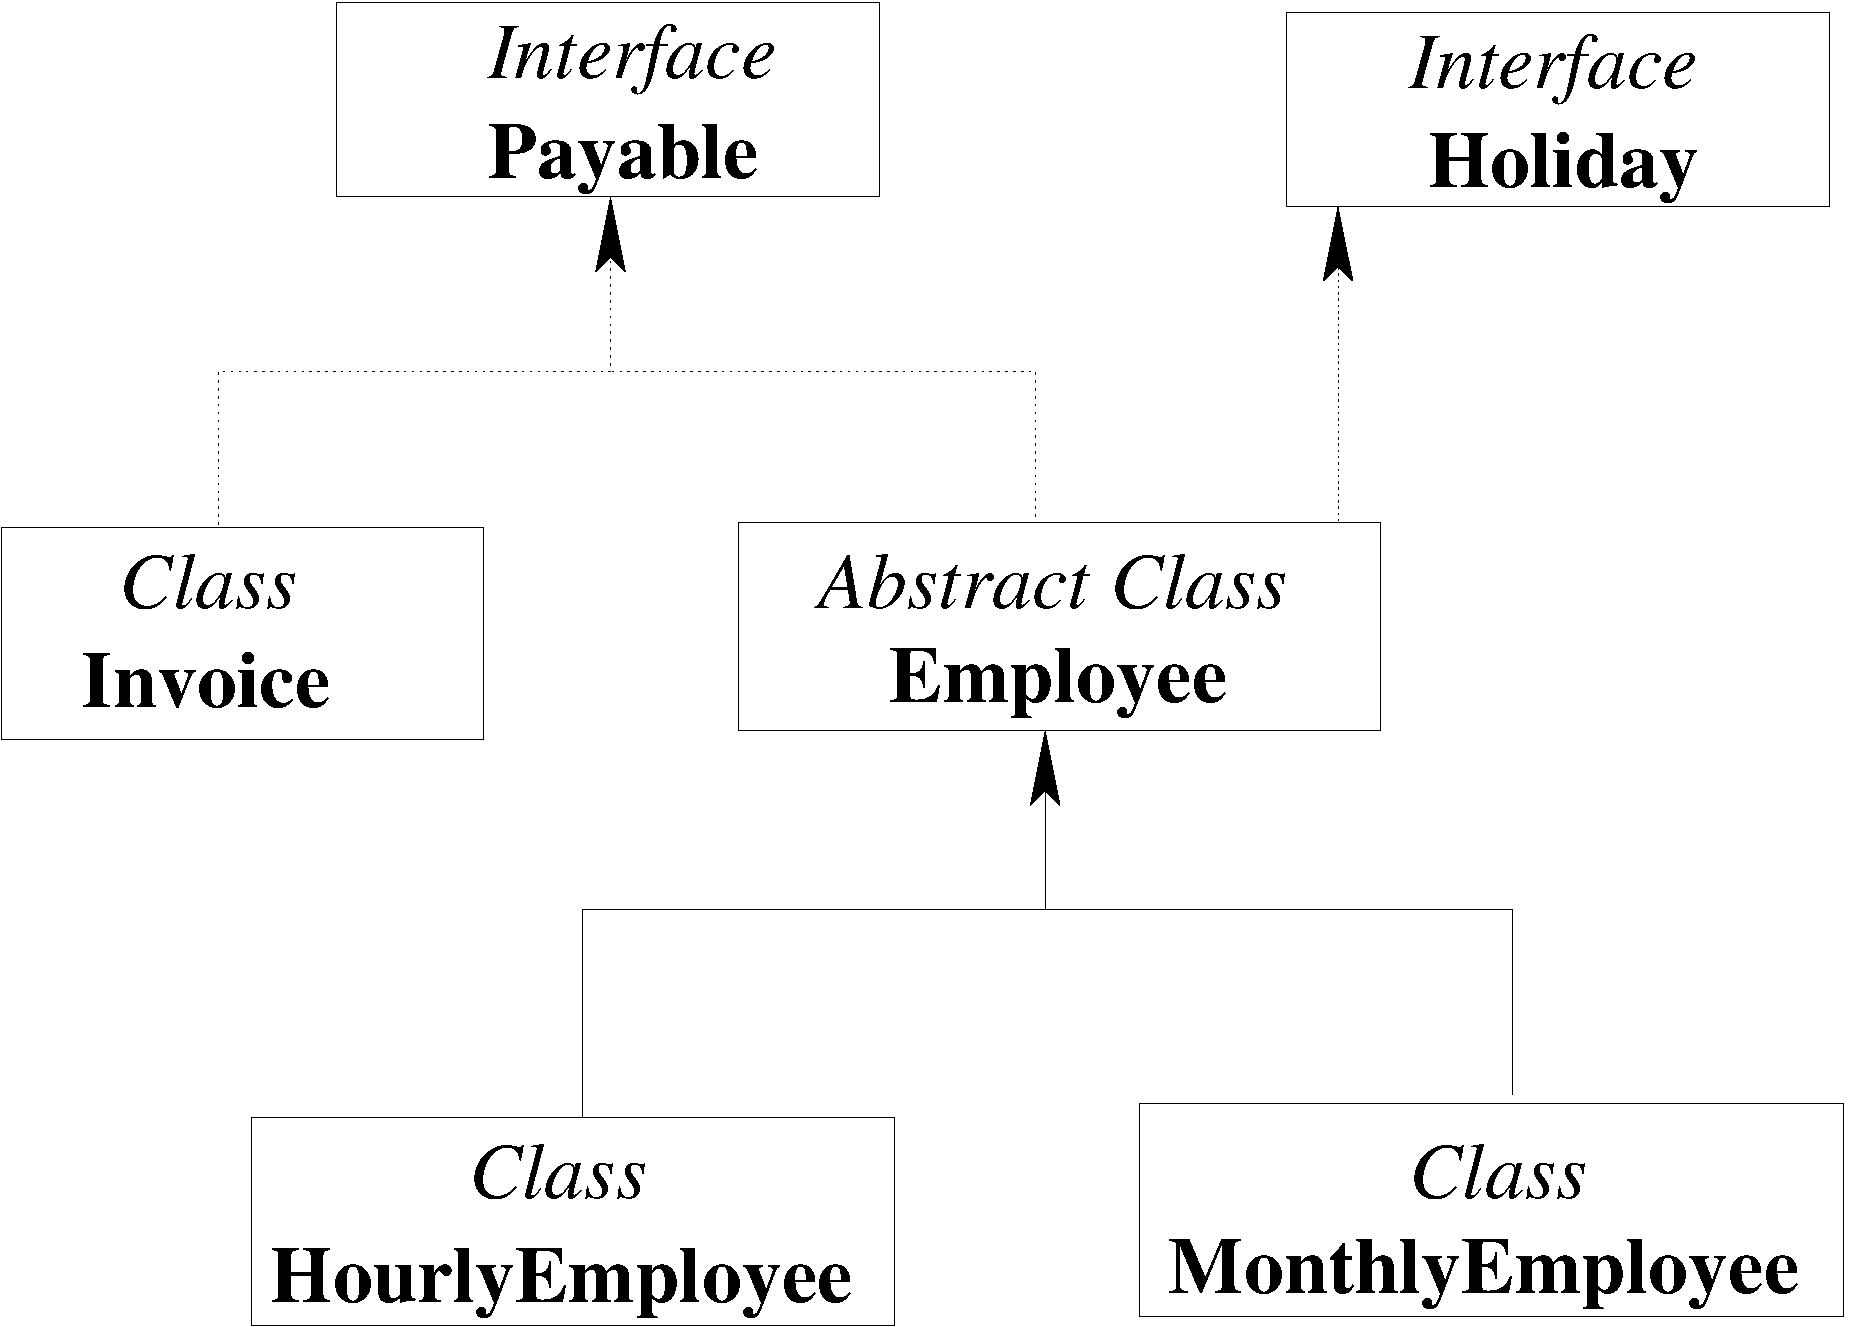
\includegraphics[height=.65\textheight]{structure}
\end{center}

\end{frame}
\begin{frame}
\frametitle{Abstract Methods} 

Just as Interfaces provide only the header of a method without an
implementation we may have in an abstract class also
\mcolor{blue}{abstract methods} for which only the header but no
implementation is given in the abstract class. In this case, it is
necessary to override the abstract method in each subclass with a
concrete method.

e.g., \mcolor{blue}{\texttt{public abstract int getPaymentAmount();}}

\end{frame}

\begin{frame}
\frametitle{\texttt{final}}

Just as variables that are declared \texttt{final}, also methods can
be declared \mcolor{blue}{\texttt{final}}. It means that they
\mcolor{red}{\textbf{CANNOT}} be overridden in a subclass.\mpause

E.g., you may want to \mcolor{blue}{disallow} in the
\texttt{BankAccount} class that the \texttt{withdraw} method is
\mcolor{blue}{overridden} from
\verbatiminput{withdraw-changed.java}
to something like
\verbatiminput{withdraw-changedTo.java}
for some subclass.
\end{frame}

\begin{frame}
\frametitle{Polymorphism}

Distinguish in inheritance whether you \mcolor{blue}{create} a new
method with \mcolor{blue}{different arguments} or
\mcolor{blue}{override an existing one} (with the same number and
types of arguments).

In superclass:
\verbatiminput{toString1.java}

Override in subclass
\verbatiminput{toString2.java}
\end{frame}

\begin{frame}
\frametitle{Polymorphism (Cont'd)}

In superclass:
\verbatiminput{toString1.java}

Is NOT overridden in subclass by
\verbatiminput{toString3.java}
\end{frame}

\begin{frame}
\frametitle{\texttt{super}}

We said that with \texttt{super} it is possible to access public
methods (and public variables) in the superclass. Note that the usage
is restricted and it is NOT possible to use e.g.
\texttt{super.super.methodName();} since this would contradict the
idea of class structuring.
\end{frame}

\begin{frame}
\frametitle{Class invariants}

[Horstmann, Big Java, p.319]:

\mcolor{blue}{``A class invariant is a statement about an object that is true after every constructor and that is preserved by every mutator (provided that the caller respects all preconditions).''} (mutator = setter)

An example is that the amount in a \texttt{BankAccount} is always bigger than or equal to 0 (or bigger than or equal to the negative overDraftLimit in a \texttt{BankAccountWithOverdraft}).

\end{frame}

\end{document}


%%% Local Variables: 
%%% mode: latex
%%% TeX-master: "slides"Superclasses
%%% End: 

